\documentclass[12pt]{article}
\usepackage[margin=2.5cm]{geometry}
\usepackage{enumerate}
\usepackage{amsfonts}
\usepackage{amsmath}
\usepackage{fancyhdr}
\usepackage{amsmath}
\usepackage{amssymb}
\usepackage{amsthm}
\usepackage{mdframed}
\usepackage{graphicx}
\usepackage{subcaption}
\usepackage{adjustbox}
\usepackage{listings}
\usepackage{xcolor}
\usepackage{booktabs}
\usepackage[utf]{kotex}
\usepackage{hyperref}

\definecolor{codegreen}{rgb}{0,0.6,0}
\definecolor{codegray}{rgb}{0.5,0.5,0.5}
\definecolor{codepurple}{rgb}{0.58,0,0.82}
\definecolor{backcolour}{rgb}{0.95,0.95,0.92}

\lstdefinestyle{mystyle}{
    backgroundcolor=\color{backcolour},
    commentstyle=\color{codegreen},
    keywordstyle=\color{magenta},
    numberstyle=\tiny\color{codegray},
    stringstyle=\color{codepurple},
    basicstyle=\ttfamily\footnotesize,
    breakatwhitespace=false,
    breaklines=true,
    captionpos=b,
    keepspaces=true,
    numbers=left,
    numbersep=5pt,
    showspaces=false,
    showstringspaces=false,
    showtabs=false,
    tabsize=1
}

\lstset{style=mystyle}

\pagestyle{fancy}
\renewcommand{\headrulewidth}{0.4pt}
\lhead{CSC 373}
\rhead{Worksheet 5 Solution}

\begin{document}
\title{CSC373 Worksheet 5 Solution}
\maketitle

\bigskip

\begin{enumerate}[1.]
    \item

    \bigskip

    \begin{proof}

    Assume that a flow network $G = (V,E)$ violates the assumption that the
    network contains a path $s \rightsquigarrow v \rightsquigarrow t$ for all
    vertices $v \in V$. Let $u$ be a vertex for which there is no path $s \rightsquigarrow u \rightsquigarrow t$.

    \bigskip

    I must show such that there is no flow at vertex $u$. That is, there exists a
    maximum flow $f$ in $G$ such that $f(u,v) = f(v,u) = 0$ for all vertices $v \in V$.

    \bigskip

    Assume for the sake of contradiction that there is some vertex $u$ with flow $f$.
    That is, there exists some vertices $v \in V$ such that $f(u,v) > 0$ or $f(v,u) > 0$.

    \bigskip

    I see that three cases follows, and I will prove each separately.

    \bigskip

    \begin{enumerate}[1.]
        \item \textbf{Cases 1:} $f(u,v) = 0$ and $f(v,u) > 0$

        \bigskip

        Here, assume that $f(u,v) = 0$ for all $v \in V$ and $f(v,u) > 0$ for some $v \in V$.

        \bigskip

        Then, we can write $\sum\limits_{v \in V} f(u,v) = 0$ and $\sum\limits_{v \in V} f(v,u) > 0$

        \bigskip

        But this violates the flow conservation property (i.e $\sum\limits_{v \in V} f(u,v) = \sum\limits_{v \in V} f(v,u)$)

        \bigskip

        Thus, by proof by contradiction, $f(u,v) = 0$ and $f(v,u) = 0$ for all $v \in V$ and
        all $u \in V$ with no path $s \rightsquigarrow u \rightsquigarrow t$.

        \bigskip

        \item \textbf{Cases 2:} $f(u,v) > 0$ and $f(v,u) = 0$

        \bigskip

        Here, assume that $f(u,v) > 0$ for some $v \in V$ and $f(v,u) = 0$ for all $v \in V$.

        \bigskip

        Then, by similar work as case 1, the same result follows.

        \bigskip

        \item \textbf{Cases 3:} $f(u,v) > 0$ and $f(v,u) > 0$

        \bigskip

        Here, assume that $f(u,v) > 0$ and $f(v,u) > 0$ for some $v \in V$.

        \bigskip

        Since $s \rightsquigarrow v \rightsquigarrow t$ and $u$ is connected by some vertices $v$,
        we can write $s \rightsquigarrow u \rightsquigarrow t$.

        \bigskip

        Then, this violates the fact in header that the vertex $u$ has no path $s \rightsquigarrow u \rightsquigarrow t$.

        \bigskip

        Thus, by proof by contradiction, $f(u,v) = 0$ and $f(v,u) = 0$ for all $v \in V$ and
        all $u \in V$ with no path $s \rightsquigarrow u \rightsquigarrow t$.

    \end{enumerate}

    \end{proof}

    \bigskip

    % \underline{\textbf{Rough Works:}}

    % \bigskip

    % Assume that a flow network $G = (V,E)$ violates the assumption that the
    % network contains a path $s \rightsquigarrow v \rightsquigarrow t$ for all
    % vertices $v \in V$. Let $u$ be a vertex for which there is no path $s \rightsquigarrow u \rightsquigarrow t$.

    % \bigskip

    % I must show such that there is no flow at vertex $u$. That is, there exists a
    % maximum flow $f$ in $G$ such that $f(u,v) = f(v,u) = 0$ for all vertices $v \in V$.

    % \bigskip

    % Assume for the sake of contradiction that there is some vertex $u$ with flow $f$.
    % That is, there exists some vertices $v \in V$ such that $f(u,v) > 0$ or $f(v,u) > 0$.

    % \bigskip

    % I see that three cases follows, and I will prove each separately.

    % \bigskip

    % \begin{enumerate}[1.]
    %     \item \textbf{Cases 1:} $f(u,v) = 0$ and $f(v,u) > 0$

    %     \bigskip

    %     Here, assume that $f(u,v) = 0$ for all $v \in V$ and $f(v,u) > 0$ for some $v \in V$.

    %     \bigskip

    %     \begin{itemize}
    %         \item Show that $\sum\limits_{v \in V} f(u,v) = 0$ and $\sum\limits_{v \in V} f(v,u) > 0$

    %         \begin{mdframed}
    %         Then, we can write $\sum\limits_{v \in V} f(u,v) = 0$ and $\sum\limits_{v \in V} f(v,u) > 0$
    %         \end{mdframed}

    %         \item Show that this violates flow conservation [contradiction]

    %         \begin{mdframed}
    %         But this violates the flow conservation property (i.e $\sum\limits_{v \in V} f(u,v) = \sum\limits_{v \in V} f(v,u)$)
    %         \end{mdframed}

    %         \item Conclude that $f(u,v) = 0$ and $f(v,u) = 0$

    %         \begin{mdframed}
    %         Thus, by proof by contradiction, $f(u,v) = 0$ and $f(v,u) = 0$ for all $v \in V$ and
    %         all $u \in V$ with no path $s \rightsquigarrow u \rightsquigarrow t$.
    %         \end{mdframed}
    %     \end{itemize}

    %     \begin{mdframed}
    %     Here, assume that $f(u,v) = 0$ for all $v \in V$ and $f(v,u) > 0$ for some $v \in V$.

    %     \bigskip

    %     Then, we can write $\sum\limits_{v \in V} f(u,v) = 0$ and $\sum\limits_{v \in V} f(v,u) > 0$

    %     \bigskip

    %     But this violates the flow conservation property (i.e $\sum\limits_{v \in V} f(u,v) = \sum\limits_{v \in V} f(v,u)$)

    %     \bigskip

    %     Thus, by proof by contradiction, $f(u,v) = 0$ and $f(v,u) = 0$ for all $v \in V$ and
    %     all $u \in V$ with no path $s \rightsquigarrow u \rightsquigarrow t$.
    %     \end{mdframed}

    %     \item \textbf{Cases 2:} $f(u,v) > 0$ and $f(v,u) = 0$

    %     \begin{mdframed}
    %     By similar work as case 1, the same result follows.
    %     \end{mdframed}

    %     \item \textbf{Cases 3:} $f(u,v) > 0$ and $f(v,u) > 0$

    %     \bigskip

    %     Here, assume that $f(u,v) > 0$ and $f(v,u) > 0$ for some $v \in V$.

    %     \bigskip

    %     \begin{itemize}
    %         \item Write that the path $s \rightsquigarrow u \rightsquigarrow t$ exists

    %         \begin{mdframed}
    %         Since $s \rightsquigarrow v \rightsquigarrow t$ and $u$ is connected by some vertices $v$,
    %         we can write $s \rightsquigarrow u \rightsquigarrow t$.
    %         \end{mdframed}

    %         \item Write that this results in contradiction to the header that
    %         a vertex $u$ has no path $s \rightsquigarrow u \rightsquigarrow t$.

    %         \begin{mdframed}
    %         Then, this violates the fact in header that the vertex $u$ has no path $s \rightsquigarrow u \rightsquigarrow t$.
    %         \end{mdframed}

    %         \item Conclude that $f(u,v) = 0$ and $f(v,u) = 0$

    %         \begin{mdframed}
    %             Thus, by proof by contradiction, $f(u,v) = 0$ and $f(v,u) = 0$ for all $v \in V$ and
    %             all $u \in V$ with no path $s \rightsquigarrow u \rightsquigarrow t$.
    %         \end{mdframed}
    %     \end{itemize}

    %     \begin{mdframed}

    %     Here, assume that $f(u,v) > 0$ and $f(v,u) > 0$ for some $v \in V$.

    %     \bigskip

    %     Since $s \rightsquigarrow v \rightsquigarrow t$ and $u$ is connected by some vertices $v$,
    %     we can write $s \rightsquigarrow u \rightsquigarrow t$.

    %     \bigskip

    %     Then, this violates the fact in header that the vertex $u$ has no path $s \rightsquigarrow u \rightsquigarrow t$.

    %     \bigskip

    %     Thus, by proof by contradiction, $f(u,v) = 0$ and $f(v,u) = 0$ for all $v \in V$ and
    %         all $u \in V$ with no path $s \rightsquigarrow u \rightsquigarrow t$.

    %     \end{mdframed}
    % \end{enumerate}

    \bigskip

    \underline{\textbf{Notes}}

    \begin{itemize}
        \item \textbf{Maximum Flow:}

        \begin{itemize}
            \item Finds a flow of maximum value $^{[1]}$

            \bigskip

            \underline{\textbf{Example}}

            \bigskip

            \begin{center}
            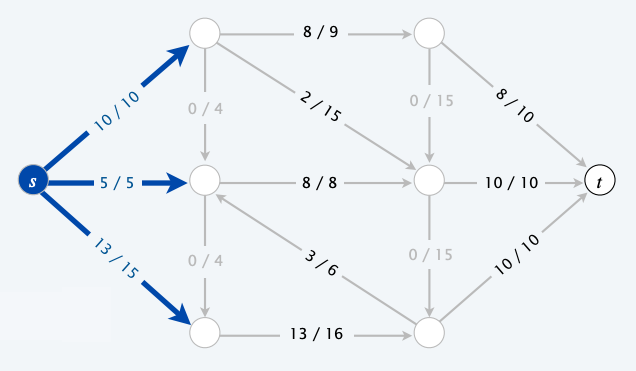
\includegraphics[width=0.7\linewidth]{images/worksheet_5_solution_3.png}
            \end{center}

            \bigskip

            Here, the maximum flow is $10 + 5 + 13 = 28$
        \end{itemize}

        \bigskip

        \item \textbf{Flow Network:}
        \begin{itemize}
            \item $G = (V,E)$ is a directed graph in which each edge $(u,v) \in E$
            has a nonnegative capacity $c(u,v) \geq 0$.
            \item Two vertices must exist: \textbf{source} s and \textbf{sink} t
            \item \textbf{path} from source $s$ to vertax $v$ to sink $t$ is represented by $s \rightsquigarrow v \rightsquigarrow t$

        \end{itemize}

        \bigskip

        \begin{center}
        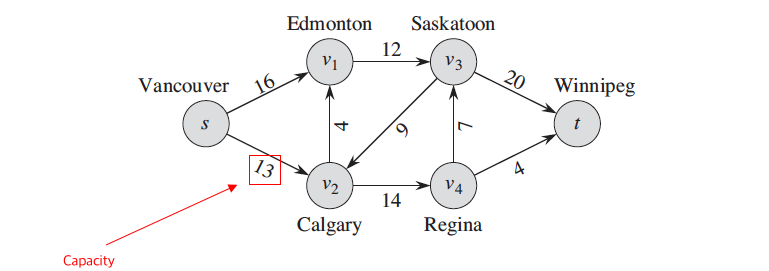
\includegraphics[width=0.9\linewidth]{images/worksheet_5_solution_1.png}
        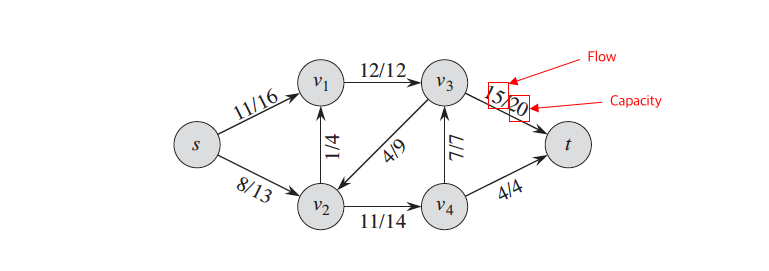
\includegraphics[width=0.9\linewidth]{images/worksheet_5_solution_2.png}
        \end{center}

        \item \textbf{Capacity:}

        \begin{itemize}
            \item Is a non-negative function $f: V \times V \to \mathbb{R}_{\geq 0}$
            \item Has \textbf{capacity constraint} where for all $u,v \in V$ $0 \leq f(u,v) \leq c(u,v)$

            \begin{itemize}
                \item Means flow cannot be above capacity constraint
            \end{itemize}
        \end{itemize}

        \item \textbf{Flow:}

        \begin{itemize}
            \item Is a real valued function $f: V \times V \to \mathbb{R}$ in $G$
            \item Satisfies \textbf{capacity constraint} (i.e for all $u,v \in V$, $0 \leq f(u,v) \leq c(u,v)$)
            \item Satisfies \textbf{flow conservation}

            \bigskip

            For all $u \in V - \{s,t\}$, we require

            \bigskip

            \begin{align}
            \sum\limits_{v \in V} f(v,u) = \sum\limits_{v \in V} f(u,v)
            \end{align}

            \bigskip

            Means flow into vertex $u$ is the same as flow going out of vertex $u$. $^{[1]}$

            \bigskip

            \underline{\textbf{Example:}}

            \begin{center}
            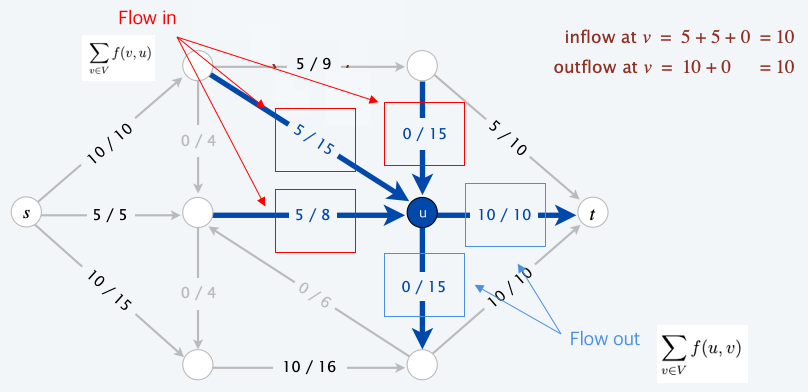
\includegraphics[width=0.9\linewidth]{images/worksheet_5_solution_4.png}
            \end{center}


        \end{itemize}
    \end{itemize}

    \bigskip

    \underline{\textbf{References}}

    \bigskip

    \begin{enumerate}[1)]
        \item Princeton University, Network Flow 1, \href{https://www.cs.princeton.edu/~wayne/kleinberg-tardos/pdf/07NetworkFlowI.pdf}{link}
    \end{enumerate}

    \item

    \bigskip

    \underline{\textbf{Rough Works:}}

    \bigskip

    I need to formulate the problem of determining whether both of professor Adam's two children can go to the same school
    as maximum-flow problem.

    \bigskip

    The problem statement tells us the following:

    \bigskip

    \begin{enumerate}[1.]
        \item There is 1 supersource (location of home)
        \item There is 1 sink (location of school)
        \item There are two sources ($s_1$ as child 1, $s_2$ as child 2)
        \item Edge $(u,v)$ has capacity of 1 (since both children cannot be on the same sidewalk)
        \item Each vertex represents corner of intersection, and two children can have their paths crossing here.
        \item Has flow of 1 or 0 (1 is where one of the two children walking on the road. 0 is none.)
    \end{enumerate}

    \bigskip

    \underline{\textbf{Notes:}}

    \bigskip

    \begin{itemize}
        \item \textbf{Cross at a Corner}

        \begin{itemize}
            \item Means to walk across the street at a corner of the intersection.

            \bigskip

            \begin{center}
            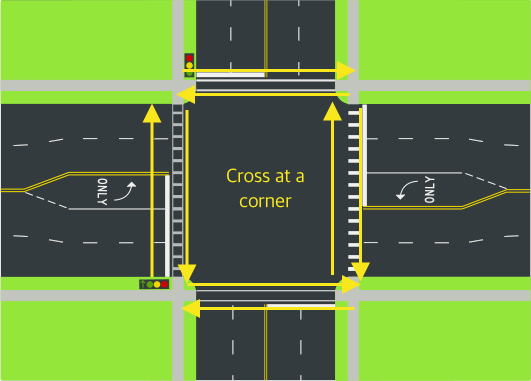
\includegraphics[width=0.7\linewidth]{images/worksheet_5_solution_5.png}
            \end{center}
        \end{itemize}

        \item \textbf{Multiple Sources and Sinks}

        \begin{itemize}
            \item Has edges $(s, s_i)$ where $i = 1 ... n$ and $(t_j, t)$ where $j = 1 ... n$
            with capacity of $\infty$
        \end{itemize}

        \bigskip

        \underline{\textbf{Example:}}

        \bigskip

        Lucky Puck Company having a set of $m$ factories $\{s_1, s_2, ..., s_m\}$, and
        a set of $n$ warehourses and $n$ warehouses $\{t_1, t_2, ..., t_n\}$

        \bigskip

        \begin{center}
        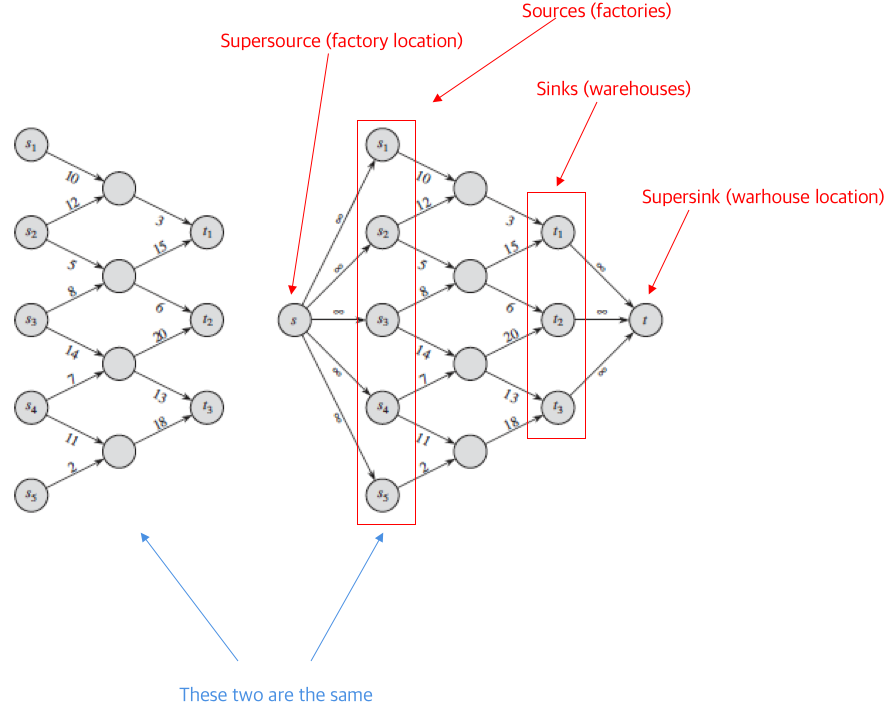
\includegraphics[width=0.9\linewidth]{images/worksheet_5_solution_6.png}
        \end{center}

    \end{itemize}

\end{enumerate}

\end{document}